%----------------------------------------------------------------------------------------
%	PACKAGES AND OTHER DOCUMENT CONFIGURATIONS
%----------------------------------------------------------------------------------------

\documentclass[twoside]{article}

\usepackage{lipsum} % Package to generate dummy text throughout this template

\usepackage[sc]{mathpazo} % Use the Palatino font
\usepackage[T1]{fontenc} % Use 8-bit encoding that has 256 glyphs
\linespread{1.05} % Line spacing - Palatino needs more space between lines
\usepackage{microtype} % Slightly tweak font spacing for aesthetics

\usepackage[hmarginratio=1:1,top=32mm,columnsep=20pt]{geometry} % Document margins
\usepackage{multicol} % Used for the two-column layout of the document
\usepackage[hang, small,labelfont=bf,up,textfont=it,up]{caption} % Custom captions under/above floats in tables or figures
\usepackage{booktabs} % Horizontal rules in tables
\usepackage{float} % Required for tables and figures in the multi-column environment - they need to be placed in specific locations with the [H] (e.g. \begin{table}[H])
\usepackage{hyperref} % For hyperlinks in the PDF

\usepackage{lettrine} % The lettrine is the first enlarged letter at the beginning of the text
\usepackage{paralist} % Used for the compactitem environment which makes bullet points with less space between them

\usepackage{abstract} % Allows abstract customization
\renewcommand{\abstractnamefont}{\normalfont\bfseries} % Set the "Abstract" text to bold
\renewcommand{\abstracttextfont}{\normalfont\small\itshape} % Set the abstract itself to small italic text

\usepackage{titlesec} % Allows customization of titles
\renewcommand\thesection{\Roman{section}} % Roman numerals for the sections
\renewcommand\thesubsection{\Roman{subsection}} % Roman numerals for subsections
\titleformat{\section}[block]{\large\scshape\centering}{\thesection.}{1em}{} % Change the look of the section titles
\titleformat{\subsection}[block]{\large}{\thesubsection.}{1em}{} % Change the look of the section titles

\usepackage{fancyhdr} % Headers and footers
\pagestyle{fancy} % All pages have headers and footers
\fancyhead{} % Blank out the default header
\fancyfoot{} % Blank out the default footer
\fancyhead[C]{ESE650 Learning in Robotics $\bullet$ March 2014 $\bullet$ Project 3} % Custom header text
\fancyfoot[RO,LE]{\thepage} % Custom footer text

\usepackage[pdftex]{graphicx}
\usepackage{epstopdf}
\usepackage{subfigure}
\usepackage{amsmath,amssymb,amsopn,amstext,amsfonts}
\usepackage{url}
\usepackage[usenames,dvipsnames]{color}
\usepackage{siunitx}
\usepackage{amsmath}
\usepackage{amsfonts}
\usepackage{amssymb}

\graphicspath{{fig/}}
\newcommand{\W}{\mathcal{W}}
\newcommand{\X}{\mathcal{X}}
\newcommand{\Y}{\mathcal{Y}}
\newcommand{\Z}{\mathcal{Z}}
\newcommand{\red}[1]{\textcolor{red}{#1}}
\newcommand{\brown}[1]{\textcolor{brown}{#1}}
%----------------------------------------------------------------------------------------
%	TITLE SECTION
%----------------------------------------------------------------------------------------

\title{\vspace{-15mm}\fontsize{24pt}{10pt}\selectfont\textbf{Gesture Recognition}} % Article title

\author{
\large
\textsc{Chao Qu}\thanks{A thank you or further information}\\[2mm] % Your name
\normalsize University of Pennsylvania \\ % Your institution
\normalsize \href{mailto:quchao@seas.upenn.edu}{quchao@seas.upenn.edu} % Your email address
\vspace{-5mm}
}
\date{}

%----------------------------------------------------------------------------------------

\usepackage{graphicx}
\begin{document}


\maketitle % Insert title

\thispagestyle{fancy} % All pages have headers and footers

%----------------------------------------------------------------------------------------
%	ABSTRACT
%----------------------------------------------------------------------------------------

%\begin{abstract}
%
%\noindent Hey, I'm just an abstract. % Dummy abstract text
%
%\end{abstract}

%----------------------------------------------------------------------------------------
%	ARTICLE CONTENTS
%----------------------------------------------------------------------------------------

%----------------------------------------------------------------------------------------
%	INTRODUCTION
%----------------------------------------------------------------------------------------

\begin{multicols}{2} % Two-column layout throughout the main article text

\section{Introduction}
\lettrine[nindent=0em,lines=2]{G}esture recognition in an interesting topic in machine learning.

%----------------------------------------------------------------------------------------
%	PRE-PROCESSING
%----------------------------------------------------------------------------------------

\section{Pre-processing}

For this project we get 9-DOF imu readings (acceleration, gyroscope and magnetometer) from a mobile phone at a sample rate of 100Hz. Although this data has been processed by the phone and has the common units, we still need to work on the data in order to use them for training and testing. The following steps are performed according to \cite{Vesa00}:

\begin{enumerate}
	\item Filter each acceleration component with fourth-order lowpass Butterworth filter with a cutoff frequency at 4Hz, see Fig.\ref{fig:imu_filt}
	\item Subsample the filtered signal at 1/5 times the original sample rate
	\item Split all the data in each gesture to a training set of 3 and valid set of 2
	\item For all the training set signal, normalize to have zero mean and unit variance and store the mean and standard deviation
	\item Cluster all training data into number number of clusters and store the centroids
\end{enumerate}

\begin{figure}[H]
\centering
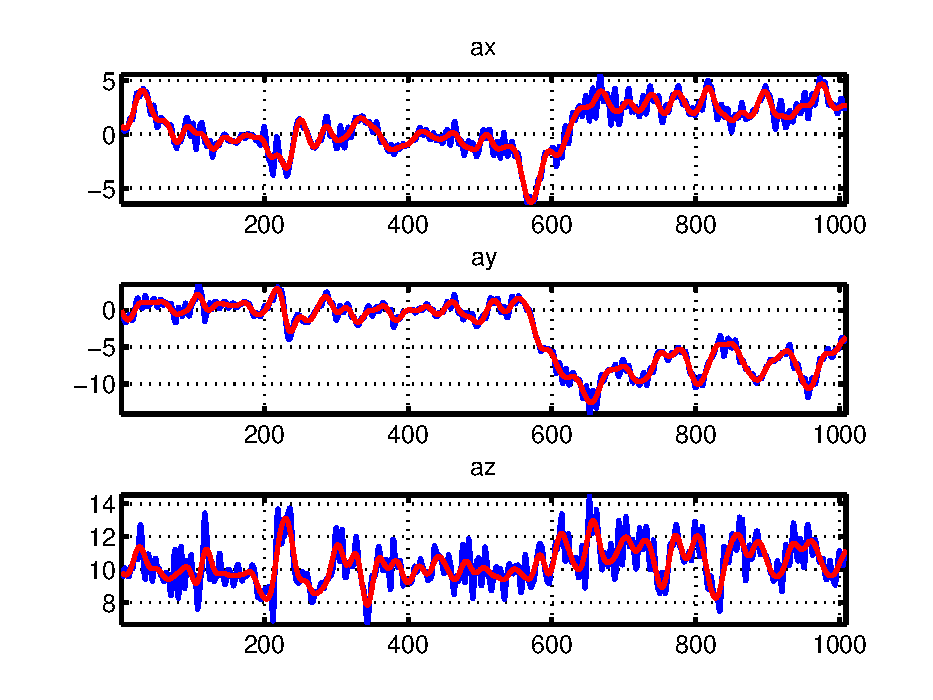
\includegraphics[width=\columnwidth]{fig/filter.pdf} 
\caption{Circle IMU data after lowpass filtering}
\label{fig:imu_filt}
\end{figure}


\begin{figure}[H]
\centering
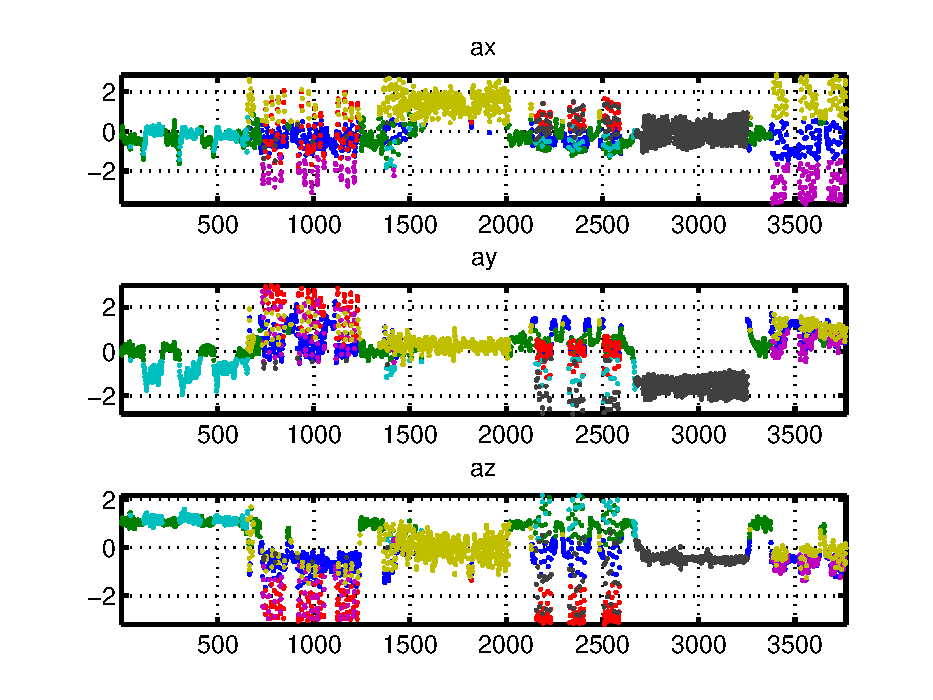
\includegraphics[width=\columnwidth]{fig/cluster.pdf} 
\caption{All training imu data after normalization and clustered}
\label{fig:imu_cluster}
\end{figure}

%----------------------------------------------------------------------------------------
%	METHODS
%----------------------------------------------------------------------------------------

\section{Methods}

%----------------------------------------------------------------------------------------
%	RESULTS
%----------------------------------------------------------------------------------------

\section{Results}


%----------------------------------------------------------------------------------------
%	DISCUSSION
%----------------------------------------------------------------------------------------

\section{Discussion}


%----------------------------------------------------------------------------------------
%	REFERENCE LIST
%----------------------------------------------------------------------------------------

\begin{thebibliography}{2} % Bibliography - this is intentionally simple in this template

\bibitem{Vesa00}
Vesa-Matti Mantyla, \emph{Hand gesture recognition of a mobile device user}. Multimedia and Expo, 2000. ICME 2000. 

%\bibitem{Cheon07}
%Y.-J. Cheon and J.-H. Kim, \emph{Unscented filtering in a unit quaternion space for spacecraft attitude estimation}. IEEE International Symposium on Industrial Electronics (ISIE 2007) (2007), pp. 66-71.
%
%\bibitem{Julier97}
%S.J. Julier, and J.K. Uhlmann, \emph{A new extension of the Kalman filter to nonlinear systems}. Proc. of AeroSense: The 11th Int. Symp. on Aerospace/Defense Sensing, Simulations and Controls, (1997).
%
\end{thebibliography}

%----------------------------------------------------------------------------------------

\end{multicols}

\end{document}
